%%%%%%%%%%%%%%%%%%%%%%%%%%%%%%%%%%%%%%%%%
% a0poster Portrait Poster
% LaTeX Template
% Version 1.0 (22/06/13)
%
% The a0poster class was created by:
% Gerlinde Kettl and Matthias Weiser (tex@kettl.de)
% 
% This template has been downloaded from:
% http://www.LaTeXTemplates.com
%
% License:
% CC BY-NC-SA 3.0 (http://creativecommons.org/licenses/by-nc-sa/3.0/)
%
%%%%%%%%%%%%%%%%%%%%%%%%%%%%%%%%%%%%%%%%%

%----------------------------------------------------------------------------------------
%	PACKAGES AND OTHER DOCUMENT CONFIGURATIONS
%----------------------------------------------------------------------------------------

\documentclass[a0,portrait]{poster}

\usepackage{multicol} % This is so we can have multiple columns of text side-by-side
\columnsep=100pt % This is the amount of white space between the columns in the poster
\columnseprule=3pt % This is the thickness of the black line between the columns in the poster

\usepackage[svgnames]{xcolor} % Specify colors by their 'svgnames', for a full list of all colors available see here: http://www.latextemplates.com/svgnames-colors

\usepackage{times} % Use the times font
%\usepackage{palatino} % Uncomment to use the Palatino font

\usepackage{graphicx} % Required for including images
\usepackage{booktabs} % Top and bottom rules for table
\usepackage[font=small,labelfont=bf]{caption} % Required for specifying captions to tables and figures
\usepackage{amsfonts, amsmath, amsthm, amssymb} % For math fonts, symbols and environments
\usepackage{wrapfig} % Allows wrapping text around tables and figures

\begin{document}

%----------------------------------------------------------------------------------------
%	POSTER HEADER 
%----------------------------------------------------------------------------------------

% The header is divided into two boxes:
% The first is 75% wide and houses the title, subtitle, names, university/organization and contact information
% The second is 25% wide and houses a logo for your university/organization or a photo of you
% The widths of these boxes can be easily edited to accommodate your content as you see fit

\begin{minipage}[b]{0.6\linewidth}
\veryHuge \color{NavyBlue} \textbf{NDNCERT in Identity Manager} \color{Black}\\ % Title
\Huge\textit{A trial to implement an identity manage using NDNCERT in Named Data Networking(NDN)}\\[2cm] % Subtitle
\huge \textbf{Yuyang(Peter) Rong, Arthi Padmanabhan, Lixia Zhang}\\[0.5cm] % Author(s)
\Large ShanghaiTech / UCLA \\ [0.4cm] % University/organization
\Large \texttt{PeterRong96@gmail.com} --- +1 (310) 307 9952\\
\end{minipage}
%
\begin{minipage}[b]{0.4\linewidth}
	
\includegraphics[width=\linewidth]{figures/logo.png}\\
\end{minipage}

\vspace{0.7cm} % A bit of extra whitespace between the header and poster content

%----------------------------------------------------------------------------------------

\begin{multicols}{2} % This is how many columns your poster will be broken into, a portrait poster is generally split into 2 columns

%----------------------------------------------------------------------------------------
%	ABSTRACT
%----------------------------------------------------------------------------------------

\color{Navy} % Navy color for the abstract

\begin{abstract}

Security and privacy in networking are gaining more and more attention nowadays. NDN proposed by Lixia Zhang has shown great potential in security. In NDN, each packet has to be signed and thus secured. In this work, we would use NDNCERT, a certificate manager, to request and manage certificates that can be used to sign data packets. We would install this manager in cell phones and thus allow other applications to gain certificate through this manager. 

\end{abstract}

%----------------------------------------------------------------------------------------
%	INTRODUCTION
%----------------------------------------------------------------------------------------

\color{SaddleBrown} % SaddleBrown color for the introduction

\section*{Introduction}
NDN requires each packet to be signed and thus can be verified. In real life applications, how they can sign their packets become a problem. Packets can be intact with the protection of self-signed signature, but it does not make the packet, nor the application, trustworthy. NDNCERT is a protocol that allows client to request a certificate that can be used to sign packets from Certificate Authority(CA). Once certificate is issued by CA, application can use that certificate to sign packets and anyone that truest the CA can trust that application. We would use NDNCERT to write a identity manager to request certificates from CA and present them to applications that are requesting it.

%----------------------------------------------------------------------------------------
%	OBJECTIVES
%----------------------------------------------------------------------------------------

\color{DarkSlateGray} % DarkSlateGray color for the rest of the content

\section*{Main Objectives}

\begin{enumerate}
\item Use NDNCERT to write identity manager;
\item Explore NDN development on Android and provide experience for other apps;
\item Provide an identity manager to update NDNFit.
\end{enumerate}

%----------------------------------------------------------------------------------------
%	MATERIALS AND METHODS
%----------------------------------------------------------------------------------------

\section*{Packages}

%------------------------------------------------

\subsection*{NDN\cite{zhang2014named}}
\par
	Unlike tradition TCP/IP architecture, in NDN every data is named under a namespace. 
	To request for a piece of data, one can express an interest with data's name inside and wait.
	When an interest is received, the corresponding data should be sent. 
	In this consumer-producer model, each and every data packet has to be signed and thus consumer can verify the integrity of the data.
\par
	Routers behavior is not our focus in this work, you can refer to the figure below or the paper cited to see how it works.
\par
\begin{minipage}[b]{0.55\linewidth}
	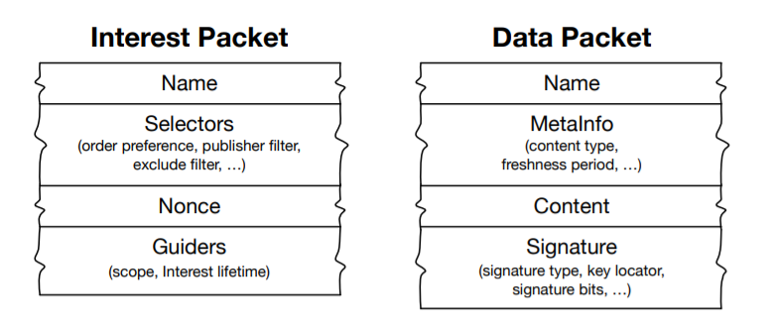
\includegraphics[width=\linewidth]{figures/packet.png}
	\captionof{figure}{packet format in NDN}
	\includegraphics[width=\linewidth]{figures/router.png}
	\captionof{figure}{router behaviors}
\end{minipage}
\begin{minipage}[b]{0.45\linewidth}
	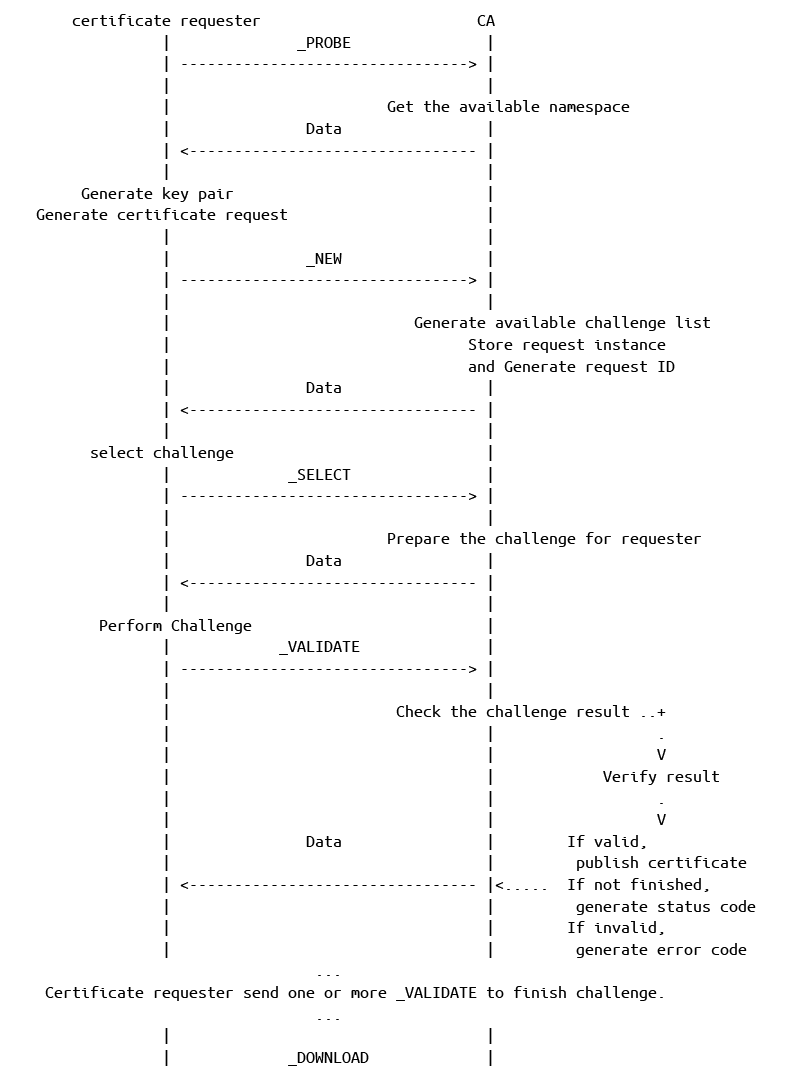
\includegraphics[width=\linewidth]{figures/protocol.png}
	\captionof{figure}{NDNCERT protocol}
\end{minipage}

%------------------------------------------------
\subsection*{NDN Certificate management protocol(NDNCERT)\cite{zhang2017ndncert}}
\par
	NDNCERT enables automatic certificate management in NDN. 
	In NDN, every entity should have corresponding identity (namespace) and the corresponding certificate for this namespace. 
	Moreover, entities need simple mechanisms to manage sub-identities and their certificates. 
	NDNCERT provides flexible mechanisms to request certificate from a certificate authority(CA) and, as soon as certificate is obtained, mechanisms to issue and manage certificates in the designated namespace.
\par
	In our project, we will be mainly focus on NDNCERT's client part. 
	As we would use NDNCERT client to get a certificate from CA and then manages these identities.
\par
	For each client to get a certificate, the steps listed in the figure above should be performed.

%------------------------------------------------
% TODO: This too.
\subsection*{Android \& Java Native Interface(JNI)}
\par 
	Applications like NDNFit require mobile clients. 
	In our case, we preferred Android over Apple, as Android are easier to develop and test.
	What's more, in the long run Android can be rooted to support NDN, yet Apple can't.
	Android has to be developed using Java, yet NDNCERT and NDN are written in c++. 
	Whether or not to use JNI has been a problem. 
	JNI provides native access to non-Java languages, allowing us to call c/c++ functions using Java. 
	In our first implementation we didn't use Java, instead we rewrote NDNCERT using Java. The benefits includes:
	\begin{itemize}
		\item No overheads for calling JNI.
		\item Easier to program/debug than JNI.
	\end{itemize}
\par
	However, soon we realized that they are downsizes too:
	\begin{itemize}
		\item Code base may be too hard to maintain. Same feature has to be implemented/ debugged twice.
	\end{itemize}
\par
	We implemented both and compared the process and the difficulty of developing.

%----------------------------------------------------------------------------------------
%	RESULTS 
%----------------------------------------------------------------------------------------

\section*{Result}
\par
Currently, the user can view details about one identity by pressing the name of the identity in the main page, or create one by pressing plus sign. The UI of certain steps in the process for apply for a new certificate is shown below. 
\par
\begin{minipage}[b]{\linewidth}
	\centering
	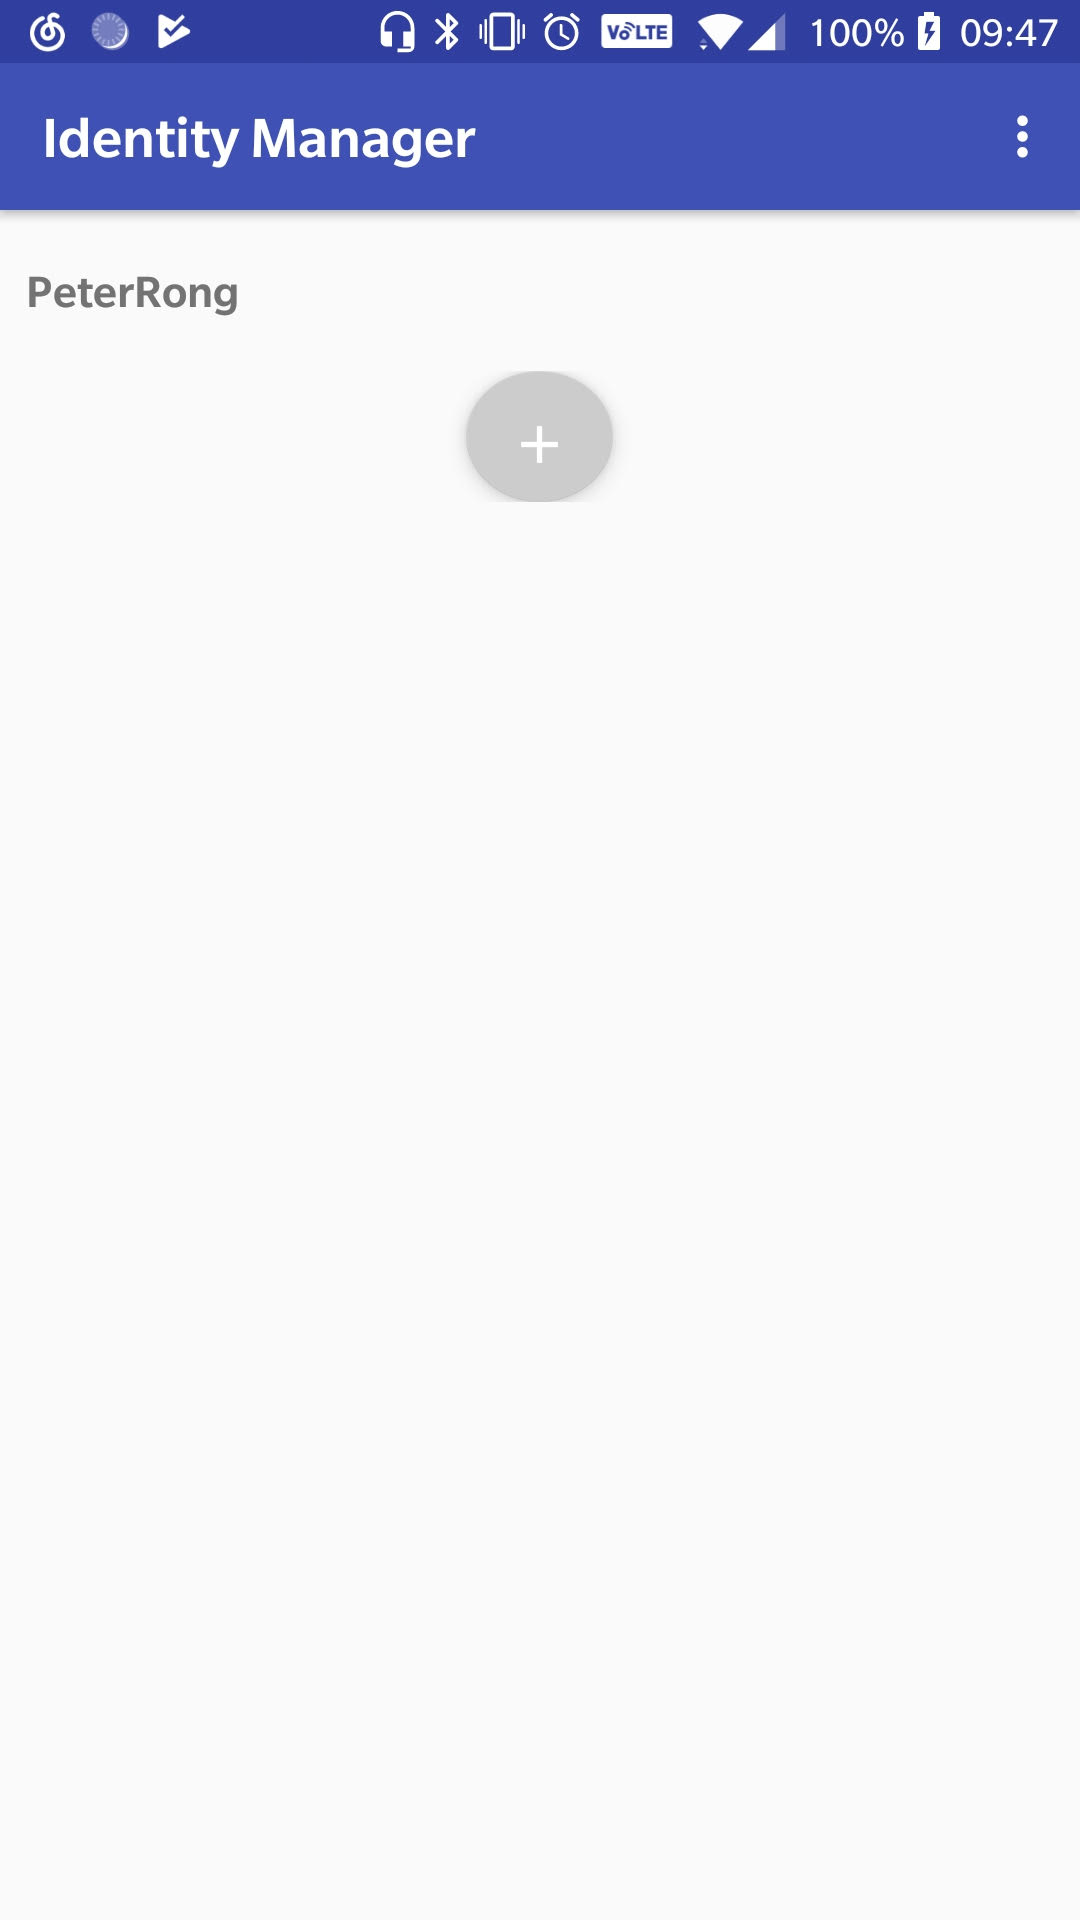
\includegraphics[width=0.24\linewidth]{figures/main-activity.jpg}
	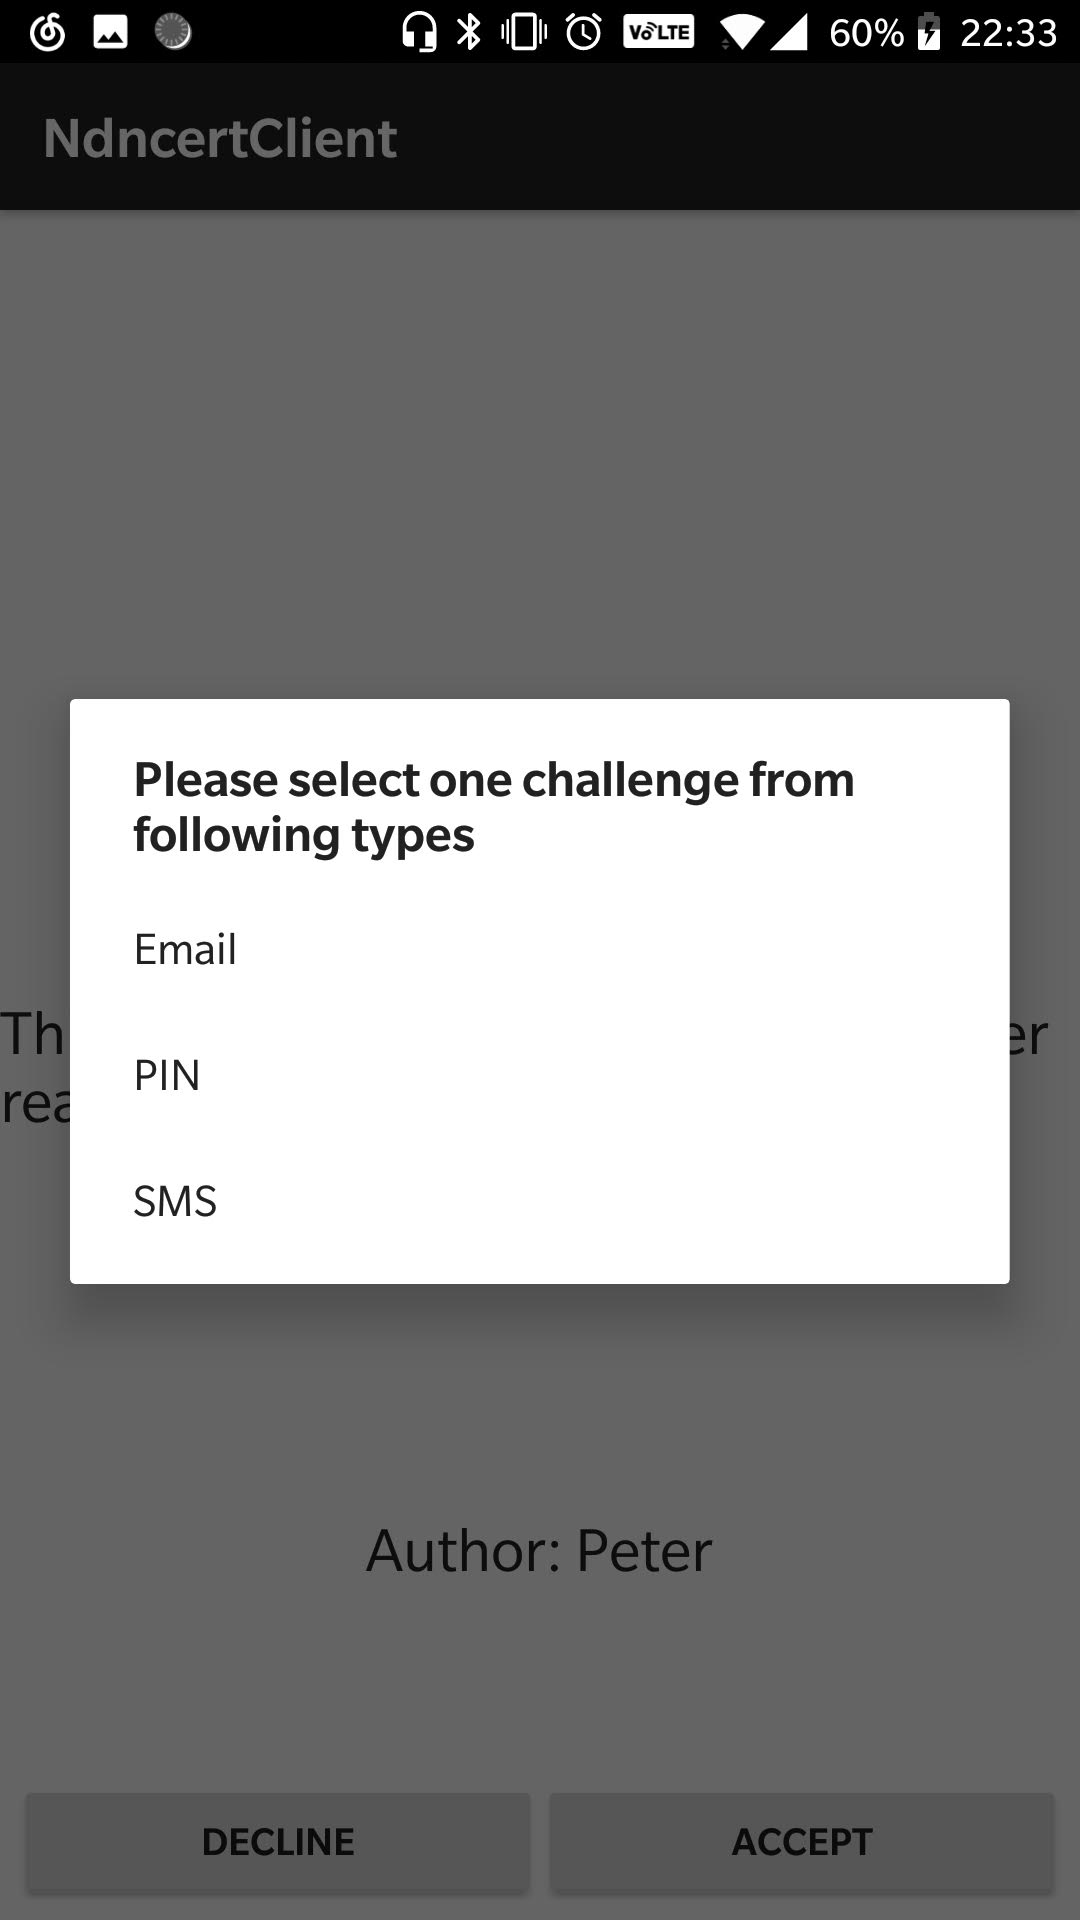
\includegraphics[width=0.24\linewidth]{figures/select.jpg}
	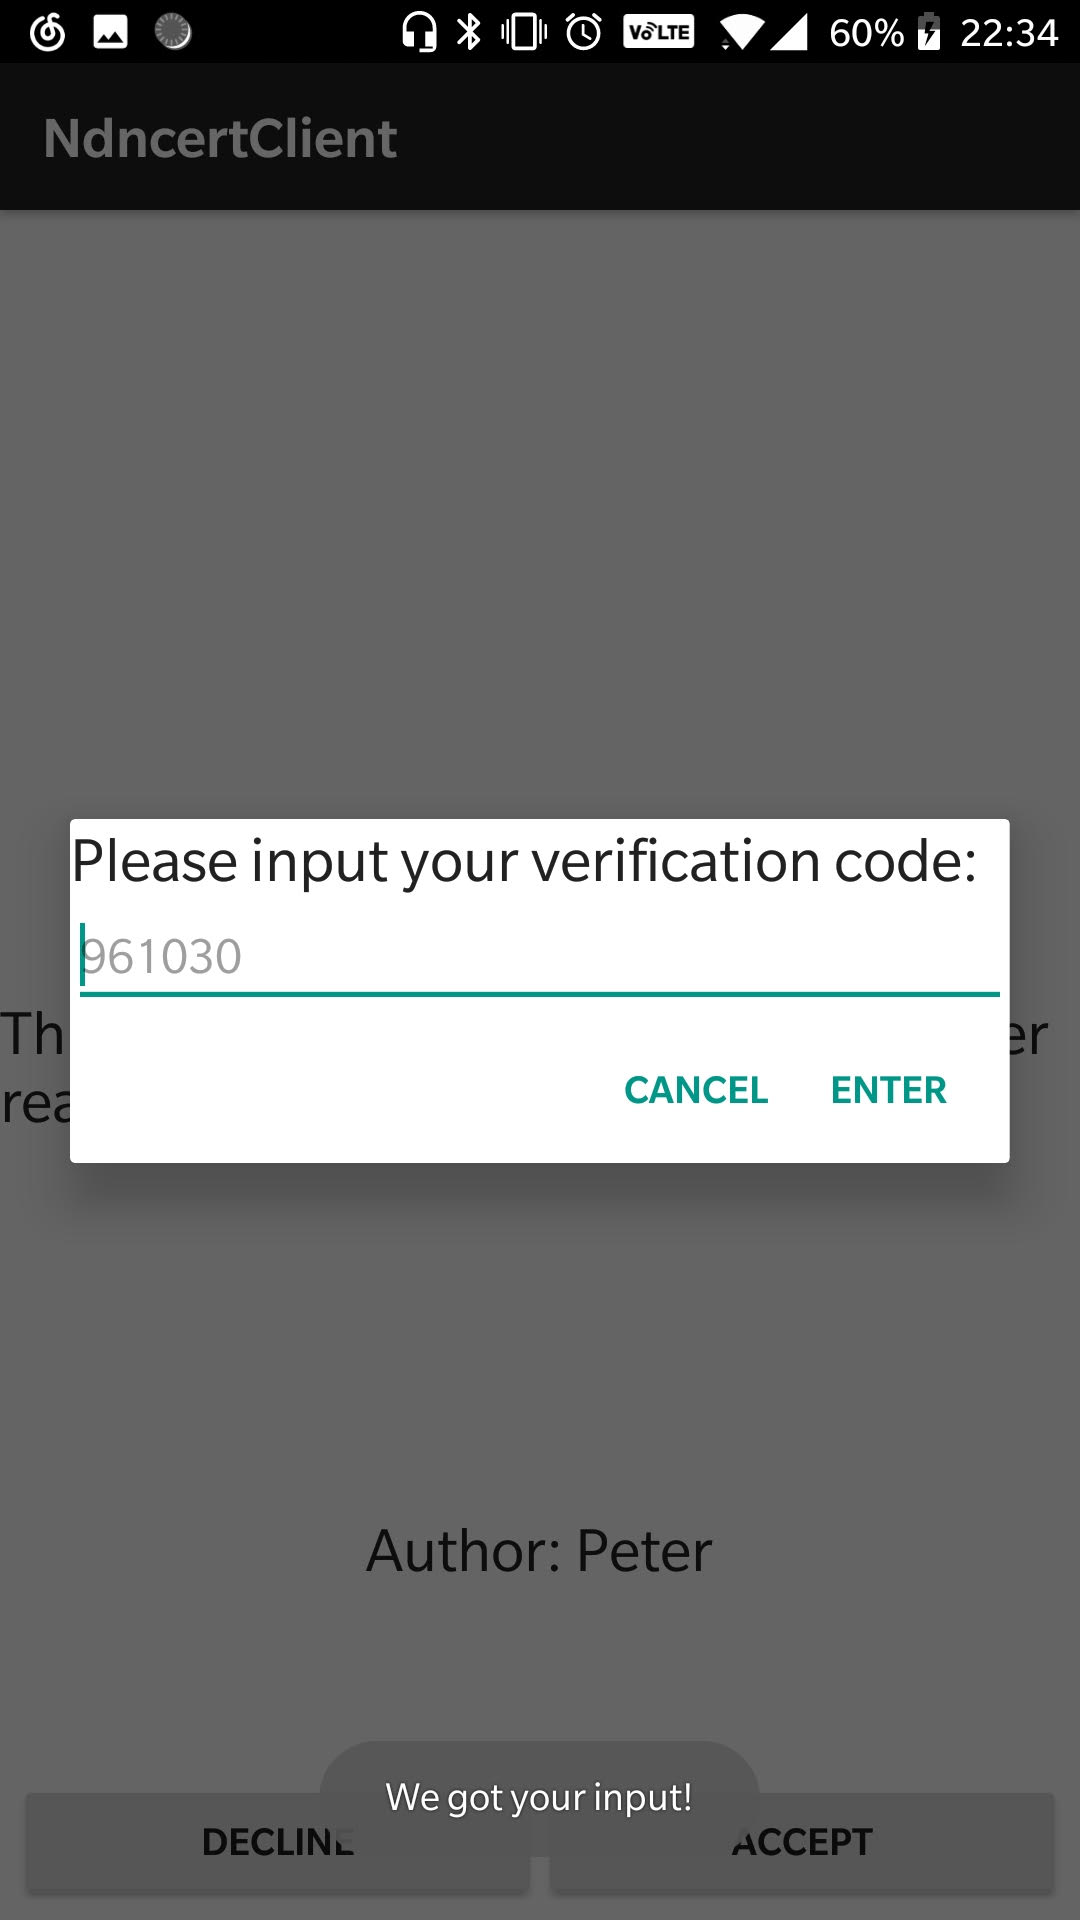
\includegraphics[width=0.24\linewidth]{figures/validate.jpg}
	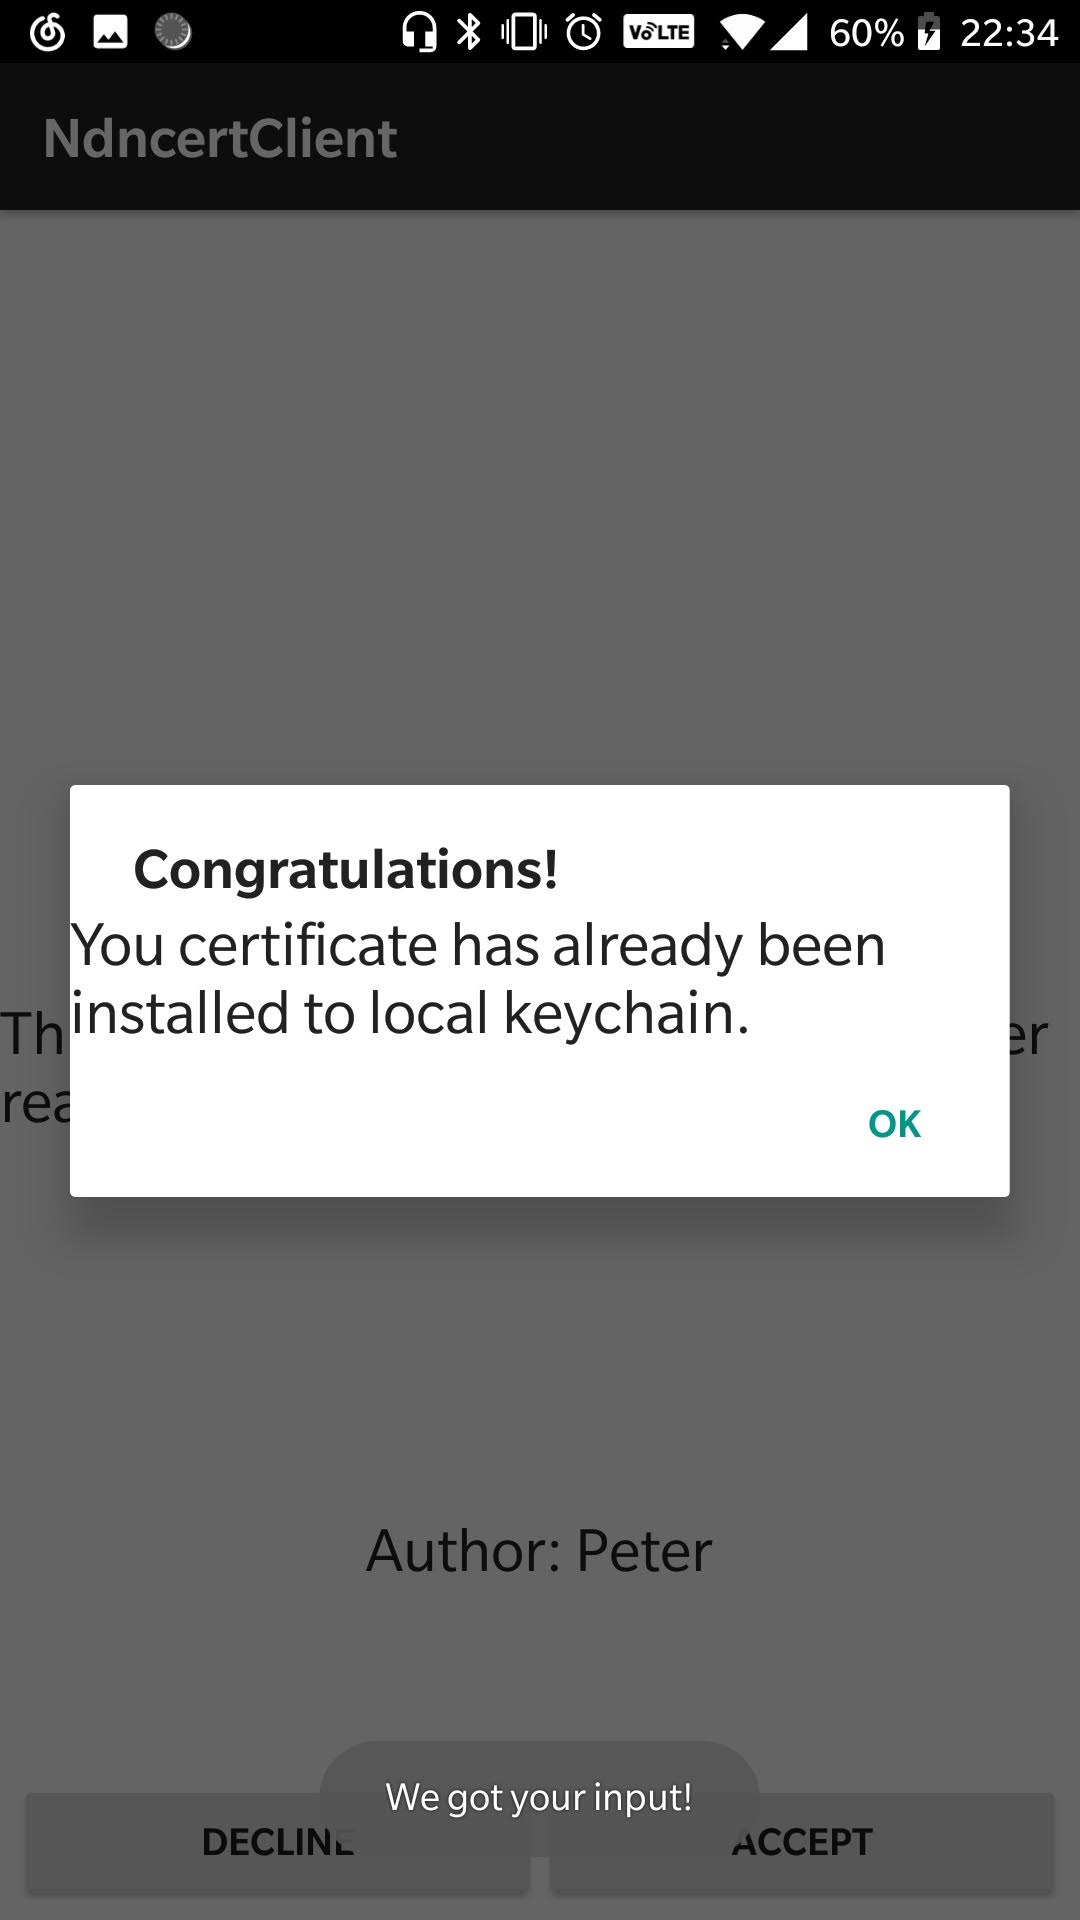
\includegraphics[width=0.24\linewidth]{figures/download.jpg}
\end{minipage}

%----------------------------------------------------------------------------------------
%	CONCLUSIONS
%----------------------------------------------------------------------------------------

%\color{SaddleBrown} % SaddleBrown color for the conclusions to make them stand out

%\section*{Conclusions}

%\color{DarkSlateGray} % Set the color back to DarkSlateGray for the rest of the content

%----------------------------------------------------------------------------------------
%	FORTHCOMING RESEARCH
%----------------------------------------------------------------------------------------

\section*{Future Work}

\par 
	Identity manager is now functional, but there are more details that can be added, including:
	\begin{itemize}
		\item identity deleting, 
		\item collision handling when identities have same name,
		\item certificate distribute when requested by other app.
	\end{itemize} 
	There are still coding to do before this app can be used by users.

%----------------------------------------------------------------------------------------
%	REFERENCES
%----------------------------------------------------------------------------------------

\nocite{*} % Print all references regardless of whether they were cited in the poster or not
\bibliographystyle{plain} % Plain referencing style
\bibliography{reference} % Use the example bibliography file sample.bib

%----------------------------------------------------------------------------------------
%	ACKNOWLEDGEMENTS
%----------------------------------------------------------------------------------------

\section*{Acknowledgments}

We would like to thank Lixia Zhang, Arthi Padmanabhan for their help and guidance. Alex Afanasyev provided a lot of help when we were developing Android application. Finally, we would like to thanks Ren Sun and CSST for providing such great opportunity.
%----------------------------------------------------------------------------------------

\end{multicols}
\end{document}